\chapter[State of the Art]{State of the Art of the Technology Used or Applied in this Thesis}

In this project, we focus on the operation of quantum simulators applied to molecular simulation, an area where quantum computing offers significant advantages. The main objective is to develop a program capable of simulating different molecules in a simple and efficient manner.

To this end, we will review the basic concepts of quantum mechanics that are essential to understand the fundamentals and potential of quantum computing, and explore the techniques of quantum simulation that allow us to harness quantum computing capabilities even with current technological limitations.

\section{Quantum Simulation}

Quantum simulation has emerged as an advanced and essential technique for studying complex quantum systems, especially those that are inaccessible or present great challenges for direct analysis using classical methods. Based on the proposal of Richard Feynman, who postulated that a computer built from quantum elements could overcome the limitations of classical computers in simulating quantum phenomena, quantum simulation has progressed significantly. It encompasses both digital and analog simulations and has expanded its applicability in various scientific areas.

There are mainly two approaches in quantum simulation: \textbf{Digital Quantum Simulation (DQS)} and \textbf{Analog Quantum Simulation (AQS)}. DQS employs the quantum circuit model, where systems are represented by qubits that evolve through quantum gates to reproduce the dynamics of the target system. This approach is universal, as it can, in principle, simulate any quantum system, although not always efficiently. On the other hand, AQS involves creating a quantum system that directly emulates the Hamiltonian of the system under study, allowing certain properties of the simulated system, such as time evolution, to be reproduced approximately. This method is particularly useful when a qualitative representation is required rather than high precision.

In addition to these approaches, there are algorithms inspired by quantum information theory that facilitate the classical simulation of quantum systems. Techniques such as \textbf{Matrix Product States (MPS)} and \textbf{Projected Entangled Pair States (PEPS)} allow representing particle systems on classical computers more efficiently than standard classical methods, optimizing the calculation of properties of complex quantum systems.

The applications of quantum simulation are broad and encompass multiple scientific fields. In condensed matter physics, it allows the study of models such as the Hubbard model and quantum phase transitions, fundamental for understanding phenomena like superconductivity. In quantum chemistry, it facilitates the calculation of molecular energies and complex chemical reactions. In high-energy physics and cosmology, it emulates particles in high-energy fields and cosmological phenomena. Furthermore, quantum simulation is instrumental in the analysis of open quantum systems and in the investigation of quantum chaos, allowing exploration of interactions with the environment and chaotic dynamics in the quantum realm.

However, quantum simulation faces significant challenges related to the precise control of the quantum simulator systems and the management of decoherence and errors, which can affect the accuracy of the results. The amount of required resources, such as the number of qubits and quantum gates, also depends on the size and complexity of the system to be simulated. It is estimated that quantum simulators require between 40 and 100 qubits to surpass the computational power of classical computers in specific problems. Despite these challenges, technological advances continue to improve the viability and efficiency of quantum simulation, promising to transform research in natural sciences and expand our understanding of quantum phenomena.

\section{Key Concepts in Quantum Mechanics}

It is essential to understand the difference between bits in classical computing and qubits in quantum computing to delve into this new technological paradigm.

In classical computing, the basic unit of information is the \textbf{bit}, which can take the value of 0 or 1. These bits are the foundation upon which conventional computers operate, processing information through combinations of these binary states.

In contrast, quantum computing uses the \textbf{qubit} or quantum bit as its basic unit. Unlike the classical bit, a qubit can exist in a superposition of states, meaning it can simultaneously represent the values 0 and 1 thanks to the principle of superposition in quantum mechanics. This property, along with phenomena such as quantum entanglement and interference, allows quantum computers to process information exponentially more efficiently for certain problems.

\begin{figure}[H]
    \centering
    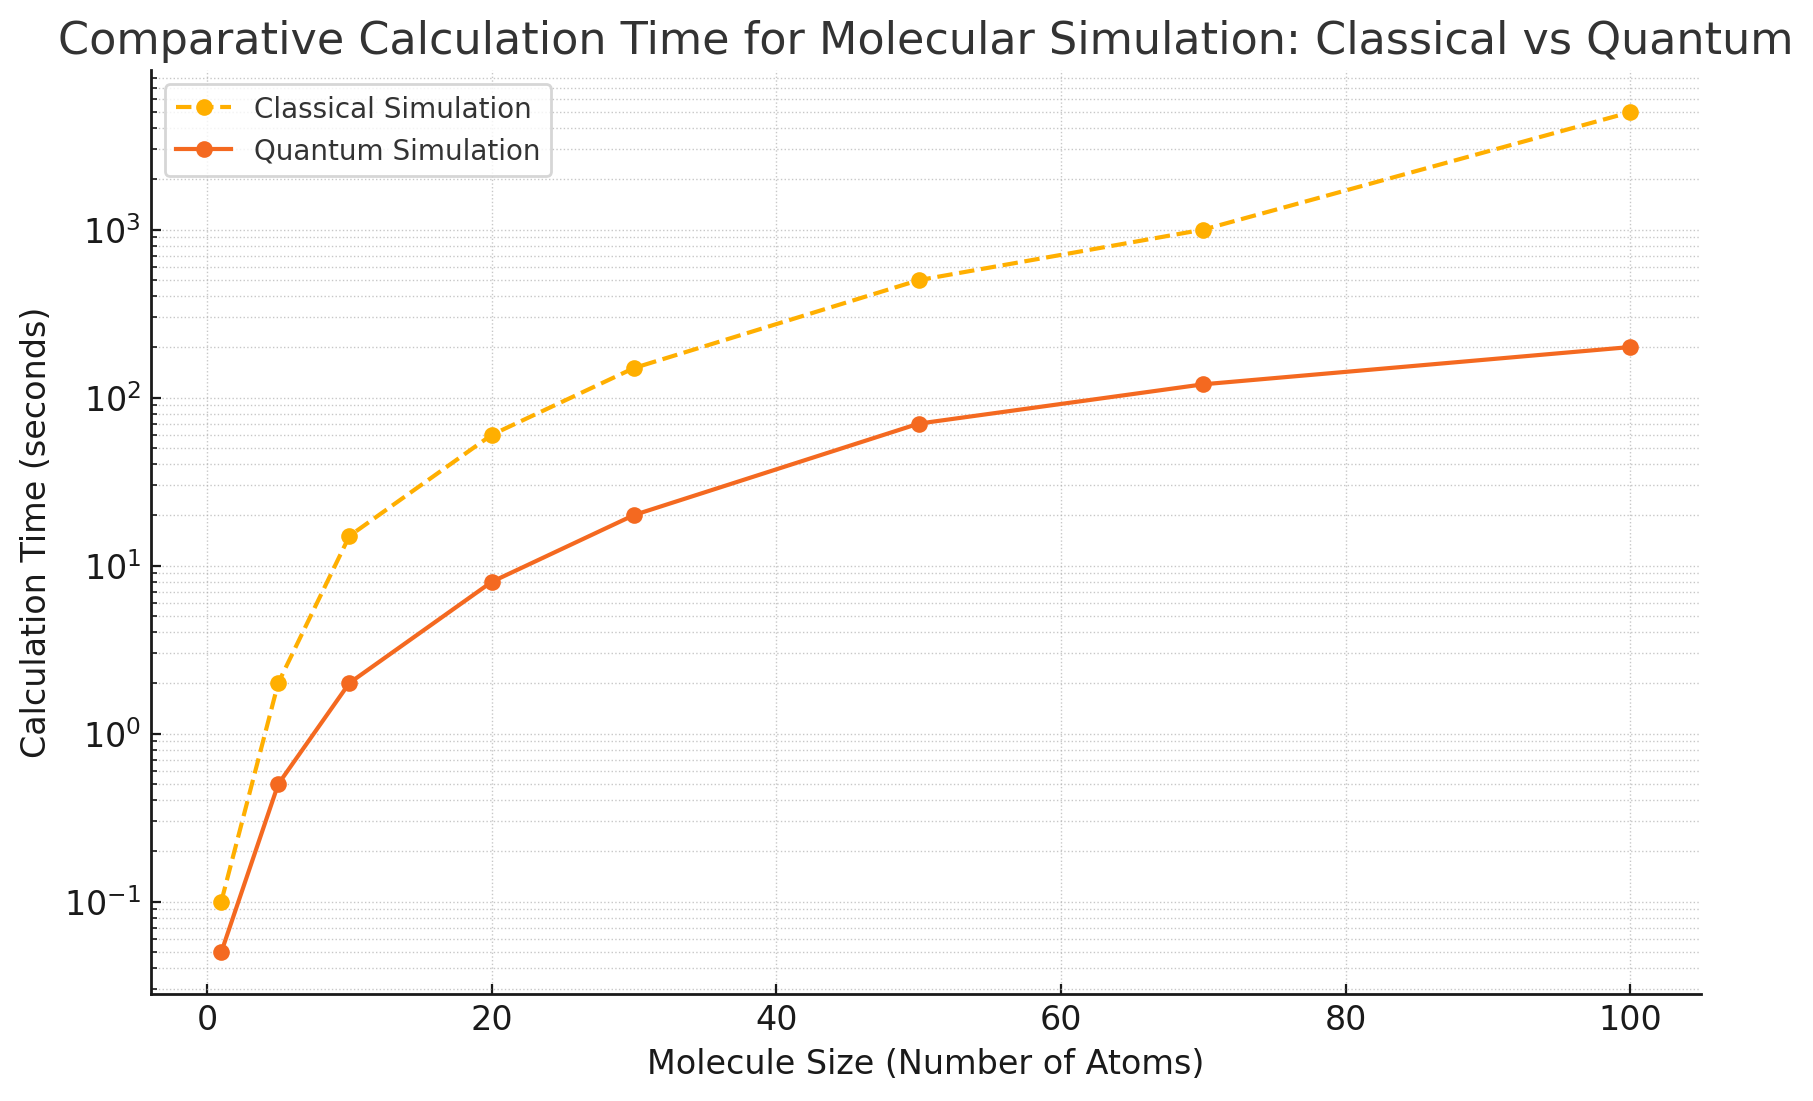
\includegraphics[width=0.8\textwidth]{img/bit_vs_qbit.png}
    \caption{Comparison of computation time for molecular simulations: classical vs quantum.}
    \label{fig:bit_vs_qubit}
\end{figure}

Understanding how qubits operate and their differences from classical bits is essential to appreciate the revolutionary potential of quantum computing.

\subsection{Qubit}

The \textbf{qubit} is the basic unit of information in quantum computing. While the classical bit can only be in one of two states (0 or 1), a qubit can be in a superposition of both states simultaneously. This is due to the principle of quantum superposition, one of the fundamental characteristics of quantum mechanics.

Mathematically, a qubit is represented as a linear combination of the basis states $\ket{0}$ and $\ket{1}$:

\[
\ket{\psi} = \alpha\ket{0} + \beta\ket{1}
\]

where $\alpha$ and $\beta$ are complex numbers that satisfy the normalization condition $|\alpha|^2 + |\beta|^2 = 1$. These coefficients indicate the probability amplitudes of finding the qubit in the states $\ket{0}$ or $\ket{1}$ upon measurement.

In addition to superposition, qubits can exhibit \textbf{quantum entanglement}, a property that allows creating strong correlations between qubits that cannot be explained by classical physics. Entanglement is essential for the computational power of quantum computers, as it enables processing and storing an exponentially larger amount of information than classical systems.

For example, while a classical system of $n$ bits can represent one of $2^n$ possible state combinations, a quantum system of $n$ qubits can represent a superposition of all those combinations simultaneously. This capability is what allows quantum computers to tackle complex problems more efficiently.

However, manipulating and maintaining qubits is a significant technical challenge. Qubits are extremely sensitive and can be affected by interactions with the environment, leading to \textbf{quantum decoherence}. To minimize this effect and preserve quantum properties, it is necessary to keep systems in controlled conditions, such as very low temperatures, close to absolute zero.

\subsection{Quantum Superposition}

\textbf{Quantum superposition} allows a quantum system to exist in multiple states simultaneously until a measurement is performed. This characteristic is key to the functioning of quantum computers, as it enables processing a large amount of information in parallel.

In quantum systems, superposition is combined with \textbf{quantum interference}, where the probability amplitudes of states can reinforce or cancel each other out. This phenomenon is exploited in quantum algorithms to increase the probability of obtaining the correct result. For example, in Grover's algorithm, constructive interference amplifies the probability of the desired state, significantly improving the efficiency of searching for elements in an unsorted database.

Superposition is especially useful in simulating complex molecular systems. Quantum computers can naturally model the superpositions of electronic states in molecules, which is crucial for studying chemical reactions and molecular properties that are difficult to address with classical methods due to the exponential growth of computational resources required.

\subsection{Quantum Decoherence}

\textbf{Quantum decoherence} is one of the main challenges in quantum computing. It refers to the loss of a system's quantum properties, such as superposition and entanglement, due to unwanted interactions with the environment. This loss causes the quantum system to transition toward classical behavior, affecting the accuracy and reliability of quantum calculations.

Qubits are extremely sensitive to external disturbances, such as electromagnetic fluctuations, vibrations, and temperature changes. These interactions can cause quantum states to mix with those of the environment, leading to a loss of coherence that is irreversible and degrades the stored quantum information.

To mitigate the effects of decoherence, various strategies are implemented:

\begin{itemize}
    \item \textbf{System Isolation}: Designing physical systems that minimize unwanted interactions with the environment, using materials and techniques that protect qubits from external disturbances.
    \item \textbf{Quantum Error Correction}: Implementing error correction codes that allow detecting and correcting errors without directly measuring the qubit's state, thereby preserving quantum information.
    \item \textbf{Dynamic Control}: Applying techniques such as pulse refocusing and dynamic pulse sequences that actively compensate for disturbances and extend the coherence time of qubits.
\end{itemize}

Controlling and mitigating decoherence are essential for the advancement of quantum computing and its application in areas like molecular simulation, where the precision of calculations is fundamental.

\section{The Hamiltonian in Quantum Mechanics}

The Hamiltonian is a fundamental concept originating from classical mechanics, introduced by William Rowan Hamilton in 1833. Hamiltonian mechanics is a reformulation of classical mechanics that provides powerful tools for studying the dynamics of systems. The Hamiltonian function represents the total energy of the system, expressed in terms of generalized coordinates and momenta, and is given by the sum of the kinetic and potential energies.

In quantum mechanics, the \textbf{Hamiltonian operator} plays a central role in describing the energy and time evolution of quantum systems. It represents the total energy of the system, including both kinetic and potential energies, and is essential for formulating the Schrödinger equation.

\subsection{Mathematical Definition}

The Hamiltonian operator, commonly denoted as \( \hat{H} \), is a self-adjoint operator acting on the Hilbert space associated with the quantum system. For a single particle in one dimension, the Hamiltonian is expressed as:

\[
\hat{H} = \hat{T} + \hat{V}
\]

where:

\begin{itemize}
    \item \( \hat{T} \) is the kinetic energy operator.
    \item \( \hat{V} \) is the potential energy operator.
\end{itemize}

In terms of the position \( \hat{x} \) and momentum \( \hat{p} \) operators, these are defined as:

\[
\hat{T} = \frac{\hat{p}^2}{2m} = -\frac{\hbar^2}{2m} \frac{d^2}{dx^2}
\]

\[
\hat{V} = V(\hat{x})
\]

Here, \( m \) is the mass of the particle, \( \hbar \) is the reduced Planck constant, and \( V(\hat{x}) \) is the potential energy function depending on position.

\subsection{Role in the Schrödinger Equation}

The Hamiltonian is central to the Schrödinger equation, which describes how the quantum state of a system evolves over time. The time-dependent Schrödinger equation is expressed as:

\[
i\hbar \frac{\partial}{\partial t} |\psi(t)\rangle = \hat{H} |\psi(t)\rangle
\]

where \( |\psi(t)\rangle \) is the state vector of the system at time \( t \). For time-independent systems, the Schrödinger equation reduces to the eigenvalue equation:

\[
\hat{H} |\psi\rangle = E |\psi\rangle
\]

Here, \( E \) represents the eigenvalues of the Hamiltonian, corresponding to the allowed energy levels of the system, and \( |\psi\rangle \) are the associated eigenstates.

\subsection{Hamiltonian in Multi-Particle Systems}

For systems with multiple particles, the Hamiltonian includes additional terms representing interactions between particles. For example, for a system of two particles, the Hamiltonian is expressed as:

\[
\hat{H} = \hat{T}_1 + \hat{T}_2 + \hat{V}_1 + \hat{V}_2 + \hat{V}_{12}
\]

where:

\begin{itemize}
    \item \( \hat{T}_1 \) and \( \hat{T}_2 \) are the kinetic energy operators of particles 1 and 2, respectively.
    \item \( \hat{V}_1 \) and \( \hat{V}_2 \) are the individual potential energy operators.
    \item \( \hat{V}_{12} \) represents the potential interaction between the two particles.
\end{itemize}

\subsection{Importance in Quantum Simulations}

In quantum simulations, especially in algorithms like the Variational Quantum Eigensolver (VQE), the Hamiltonian is decomposed into a sum of simpler terms, often expressed in terms of Pauli operators. This decomposition facilitates implementation on quantum circuits and allows estimating the system's energy through measurements on qubits.

Understanding the structure and properties of the Hamiltonian is essential for modeling and simulating quantum systems, as it determines the possible energies and dynamics of the system under study.

\section{VQE: Variational Quantum Eigensolver}
\label{sec:vqe}

Among the hybrid quantum-classical algorithms developed to address quantum simulation challenges, the \emph{Variational Quantum Eigensolver (VQE)} has gained particular relevance. This method seeks to approximate the ground-state energy of a target Hamiltonian, such as the electronic Hamiltonian of a molecule, by efficiently combining quantum state preparation with classical optimization techniques.

\subsection{Fundamental Principles and Stages of the Algorithm}
\label{subsec:vqe_principles_stages}

VQE is founded on the \textbf{variational principle} of quantum mechanics, which states that the expectation value of the energy 
\(\,E(\vec{\theta})\)
for any normalized trial state \(\,\ket{\psi(\vec{\theta})}\) is always an upper bound to the true ground-state energy \(E_0\):
\[
E(\vec{\theta}) 
= \bra{\psi(\vec{\theta})} \hat{H} \ket{\psi(\vec{\theta})}
\;\;\geq\; E_0.
\]
Because \(E(\vec{\theta})\) depends on a set of parameters \(\vec{\theta}\), the VQE algorithm iteratively updates these parameters to minimize \(E(\vec{\theta})\). Once no further reduction in \(E(\vec{\theta})\) is possible, the algorithm identifies the lowest value reached as an approximation of \(E_0\).

In practice, VQE proceeds in a loop that integrates quantum and classical resources:

\begin{enumerate}
    \item \textbf{Quantum State Preparation:} 
    A parameterized quantum circuit, commonly termed an \emph{ansatz}, is constructed with a set of adjustable parameters \(\vec{\theta}\). This circuit leverages unitary gates (e.g., single-qubit rotations, entangling gates) to create a trial wavefunction:
    \[
    \ket{\psi(\vec{\theta})}.
    \]

    \item \textbf{Measurement of the Expected Energy:}
    The Hamiltonian \(\hat{H}\) is decomposed into a sum of Pauli operators acting on the qubits. The expectation value 
    \(\langle \psi(\vec{\theta}) \mid \hat{H} \mid \psi(\vec{\theta}) \rangle\)
    is obtained by measuring the appropriate Pauli operators on the quantum device, typically requiring multiple circuit executions due to non-commuting terms.

    \item \textbf{Classical Optimization:}
    The measured energy serves as a cost function, \(E(\vec{\theta})\). A classical optimizer---such as \emph{Gradient Descent} or \emph{Adam}---then updates the parameters \(\vec{\theta}\) to minimize this cost.

    \item \textbf{Iteration and Convergence:}
    Steps 1--3 repeat until a convergence criterion is satisfied, for instance,
    \[
    \left|\,E\bigl(\vec{\theta}_{k+1}\bigr) - E\bigl(\vec{\theta}_{k}\bigr)\right|
    \;<\;\delta,
    \]
    where \(\delta\) is a small threshold for energy differences. The final set \(\vec{\theta}^{*}\) yields an approximate ground-state wavefunction and energy.
\end{enumerate}

\subsection{Advantages and Challenges}
\label{subsec:vqe_challenges}

VQE has garnered extensive interest in fields like \textbf{quantum chemistry}, \textbf{materials science}, and even combinatorial optimization problems mapped to Hamiltonians. Its hybrid structure allows leveraging near-term quantum devices (with limited qubits and gate depths) while offloading resource-intensive tasks---such as parameter updates---to classical computers. 

Despite its promise, VQE faces several practical hurdles:

\begin{itemize}
    \item \textbf{Noise and Decoherence:} 
    Real quantum devices suffer from errors that deteriorate the fidelity of prepared states and measurements, requiring error-mitigation strategies and noise-aware ansatz designs.

    \item \textbf{Barren Plateaus:}
    High-dimensional parameter spaces can contain large regions where gradients vanish, complicating the search for global minima.

    \item \textbf{Measurement Overhead:}
    Decomposing a Hamiltonian into many Pauli terms demands running multiple circuits, increasing sampling time and exposure to hardware noise.

    \item \textbf{Circuit Depth:}
    Accurate ans\"atze for complex systems may require deep circuits that quickly exceed the coherence times of current quantum processors.
\end{itemize}

\subsection{Outlook in Quantum Simulation}
\label{subsec:vqe_outlook}

Continuous improvements in both hardware (qubit quality, gate fidelity, and error-correction schemes) and software (advanced ans\"atze, better optimizers, error mitigation) keep driving VQE toward practical applications. Recent strategies such as \emph{ADAPT-VQE}, which adaptively builds up an excitation operator set, and domain-specific ans\"atze integrated with error mitigation methods, further enhance VQE’s accuracy for molecular systems. 

As the number of qubits grows and quantum hardware matures, VQE is likely to become a central approach for tackling classically intractable problems in quantum chemistry, materials science, and beyond. Its flexible hybrid nature will continue to serve as a testbed for new optimization algorithms, ansatz designs, and measurement strategies, bridging current \emph{Noisy Intermediate-Scale Quantum (NISQ)} devices with the longer-term ambition of fault-tolerant quantum computing.

\section{Different Ans\"{a}tze in Quantum Chemistry and Quantum Computing}
In the context of variational quantum algorithms and quantum chemistry, an \textbf{ansatz} is a carefully chosen, often physically motivated, parametric form of the quantum state used to approximate the ground (or excited) state of a system described by a given Hamiltonian. The term \textit{ansatz} originates from the German word \textquotedblleft approach\textquotedblright\ or \textquotedblleft initial guess,\textquotedblright\ and it reflects the central idea that we propose a functional form (or circuit structure) for the wavefunction and then optimize the parameters in search of the lowest possible energy. 

Within the framework of the Variational Quantum Eigensolver (VQE), the ansatz is implemented as a parameterized quantum circuit whose gates depend on a set of continuous variables $\vec{\theta}$. By measuring the expectation value of the Hamiltonian with respect to this trial state, one obtains an energy estimate $E(\vec{\theta})$ which is then iteratively minimized by a classical optimizer. The success of a VQE calculation hinges critically on the expressiveness and resource requirements (number of gates, circuit depth, etc.) of the chosen ansatz.

Several ans\"{a}tze have been proposed to achieve a balance between accuracy and computational cost. Below, we summarize the most relevant approaches, highlighting their theoretical underpinnings and current usage in quantum simulation.

\subsection{Hartree--Fock-based Ans\"{a}tze (Classical Reference)}
A historically important \textquotedblleft classical\textquotedblright\ ansatz in quantum chemistry arises from the \textbf{Hartree--Fock (HF)} approximation. In this method, the total wavefunction is assumed to be a single Slater determinant constructed from one-particle orbitals. Although it captures the fundamental antisymmetry required by the Pauli exclusion principle (i.e., fermionic exchange), it neglects most of the electron correlation. Post-HF methods, such as Configuration Interaction (CI), Many-Body Perturbation Theory (MPn), and Coupled Cluster (CC), then build on this reference state by introducing additional terms that account for electron correlation.  

\begin{itemize}
    \item \textbf{Configuration Interaction (CI):} Expands the wavefunction in a basis of Slater determinants (excitations) beyond the HF reference. The Full CI approach is exact within the chosen basis but scales exponentially with system size. Truncated CI methods (CIS, CID, CISD, etc.) reduce the computational cost but still grow quickly with system size.

    \item \textbf{Coupled Cluster (CC):} Expresses the wavefunction via an exponential of excitation operators acting on the HF reference. Formally written as 
    \[
       |\Psi_{\mathrm{CC}}\rangle = e^{\hat{T}}|\Phi_{\mathrm{HF}}\rangle,
    \]
    where $\hat{T}$ is the sum of cluster excitation operators (singles, doubles, triples, etc.). Although Coupled Cluster with Singles and Doubles (CCSD) is often accurate, further inclusion of triples and higher excitations can be required for strongly correlated systems.
\end{itemize}

In the context of classical methods, these \textbf{ans\"{a}tze} serve as trial wavefunctions whose coefficients are optimized using high-performance classical algorithms. Their conceptual basis---constructing physically motivated trial states that capture crucial features of the system---carries over into quantum computing.

\subsection{Unitary Coupled Cluster (UCC)}
A key adaptation of the Coupled Cluster theory to quantum computing is the \textbf{Unitary Coupled Cluster (UCC)} ansatz. It modifies the standard CC exponential by making it explicitly unitary:

\[
|\Psi_{\mathrm{UCC}}\rangle 
= e^{\hat{T}(\vec{\theta}) - \hat{T}^\dagger(\vec{\theta})} \,|\Phi_{\mathrm{HF}}\rangle,
\]

where $\hat{T}(\vec{\theta})$ is typically truncated to include only single and double excitations (UCCSD). This approach guarantees that the resulting operator is unitary, which is crucial for hardware implementations in quantum computing since all gates must be unitary transformations. 

\begin{itemize}
    \item \textbf{UCCSD (Singles and Doubles):} The most widespread version of UCC is truncated at single and double excitations:
    \[
        \hat{T}(\vec{\theta}) = \sum_{i,a} \theta_{i}^{a} \hat{a}_a^\dagger \hat{a}_i 
          \,\,+\,\, 
          \sum_{i,j,a,b} \theta_{i,j}^{a,b} \hat{a}_a^\dagger \hat{a}_b^\dagger \hat{a}_j \hat{a}_i
          \,\,+\, \cdots
    \]
    Here, $i, j$ denote occupied orbitals and $a, b$ virtual (unoccupied) orbitals. By exponentiating both $\hat{T}$ and $\hat{T}^\dagger$, the wavefunction stays normalized. However, the circuit depth can become large since implementing the exponential of a sum of non-commuting operators requires a trotterization or related approximation.

    \item \textbf{ADAPT-VQE and Variants:} To mitigate the high circuit cost, variants like \textit{ADAPT-VQE} build up a UCC-type ansatz incrementally, selecting only those excitation operators that most significantly lower the energy at each step. This adaptive approach reduces the number of gates needed and often converges faster.
\end{itemize}

\subsection{Problem-Inspired or Custom Ans\"{a}tze}
In some cases, \textbf{custom ans\"{a}tze} are tailored to the specific physical or chemical system under investigation. For example, if certain symmetries (like particle number or spin) are known to be crucial for describing the ground state, one can design an ansatz that explicitly respects those symmetries. Such approaches can drastically reduce the parameter space and improve convergence, albeit with some additional effort in circuit design.

\section{Optimizers}
\label{sec:optimizers}

In quantum simulation algorithms such as the Variational Quantum Eigensolver (VQE), optimizers constitute a key element of the hybrid quantum-classical workflow. Their primary objective is to minimize the cost function
\[
E(\vec{\theta}) = \langle \psi(\vec{\theta}) \mid \hat{H} \mid \psi(\vec{\theta}) \rangle,
\]
where \(\hat{H}\) represents the Hamiltonian of the system under study and \(\ket{\psi(\vec{\theta})}\) is a parameterized quantum state, often referred to as the \emph{ansatz}. After each quantum measurement, the optimizer updates the parameter vector \(\vec{\theta}\) to guide the system toward the ground-state energy. This process is iterated until convergence, balancing the capabilities of quantum hardware with classical numerical techniques.

In the following subsections, we discuss the theoretical underpinnings and key features of several optimizers commonly employed in variational algorithms. While all these optimizers share the goal of efficiently navigating the parameter space, they differ in how they incorporate gradients, memory of past iterations, and adjustments of the learning rate.

\subsection{Gradient Descent (GD)}
\label{subsec:gd}
\emph{Gradient Descent} is one of the most fundamental methods for continuous optimization. At each iteration, it updates parameters by moving them in the direction opposite to the gradient of the cost function:
\[
\vec{\theta}_{k+1} = \vec{\theta}_{k} 
- \eta \nabla_{\vec{\theta}} E(\vec{\theta}_{k}),
\]
where \(\eta\) is the learning rate and \(\nabla_{\vec{\theta}} E(\vec{\theta})\) denotes the gradient of the cost function with respect to the parameters. Despite its simplicity, Gradient Descent can converge slowly or get trapped in local minima when dealing with complex or high-dimensional landscapes, making it less efficient if used alone in large-scale molecular simulations.

\subsection{Momentum Optimizer}
\label{subsec:momentum}
The \emph{Momentum} method extends standard Gradient Descent by incorporating a velocity term that accumulates a fraction of previous updates. This approach can mitigate oscillations and speed up convergence in regions with shallow gradients. The update rule is given by:
\[
\begin{aligned}
\vec{v}_{k+1} &= \gamma \vec{v}_{k} 
- \eta \nabla_{\vec{\theta}} E(\vec{\theta}_{k}),\\
\vec{\theta}_{k+1} &= \vec{\theta}_{k} + \vec{v}_{k+1},
\end{aligned}
\]
where \(\gamma\) (typically between 0.9 and 0.99) is the momentum coefficient that controls how much past gradients influence the current update. This optimizer often accelerates learning in practice by effectively smoothing noisy or rapidly changing gradients.

\subsection{Nesterov Momentum Optimizer (NMomentum)}
\label{subsec:nmomentum}
\emph{Nesterov Momentum}, sometimes referred to as \emph{Nesterov’s Accelerated Gradient (NAG)}, refines the idea of Momentum by anticipating the next position of the parameters before computing the gradient. Concretely, one computes the gradient at \(\vec{\theta} + \gamma \vec{v}\) rather than at \(\vec{\theta}\) only. The updates become:
\[
\begin{aligned}
\vec{v}_{k+1} &= \gamma \vec{v}_{k} 
- \eta \nabla_{\vec{\theta}}
E\!\big(\vec{\theta}_{k} + \gamma \vec{v}_{k}\big),\\
\vec{\theta}_{k+1} &= \vec{\theta}_{k} + \vec{v}_{k+1}.
\end{aligned}
\]
By \textquoteleft looking ahead\textquoteright\ in the direction of the velocity term, Nesterov Momentum tends to achieve smoother convergence and better performance on problems with numerous local minima or saddle points, which are common in complex quantum simulations.

\subsection{RMSProp}
\label{subsec:rmsprop}
\emph{RMSProp} is a gradient-based optimizer that adaptively tunes the learning rate for each parameter by normalizing the gradient through a moving average of its recent magnitudes. This helps address issues of vanishing or exploding gradients, which can be particularly troublesome in variational circuits of moderate or large depth. Its core update equations are:
\[
\begin{aligned}
E[\nabla^2_{\vec{\theta}}]_{k} &= \beta \, E[\nabla^2_{\vec{\theta}}]_{k-1}
+ (1-\beta)\,\nabla_{\vec{\theta}} E(\vec{\theta}_{k})^2,\\
\vec{\theta}_{k+1} &= \vec{\theta}_{k} 
- \eta \, \frac{\nabla_{\vec{\theta}} E(\vec{\theta}_{k})}
{\sqrt{E[\nabla^2_{\vec{\theta}}]_{k}} + \epsilon},
\end{aligned}
\]
where \(0 < \beta < 1\) is a decay factor controlling the smoothing effect, and \(\epsilon\) is a small constant ensuring numerical stability.

\subsection{Adagrad}
\label{subsec:adagrad}
\emph{Adagrad} is an early approach to adaptive learning rates, designed to handle sparse or highly non-uniform gradients. It individually scales the updates by the inverse square root of the cumulative sum of gradients:
\[
\vec{\theta}_{k+1} 
= \vec{\theta}_{k} 
- \frac{\eta}{\sqrt{\sum_{i=1}^{k} 
  \nabla_{\vec{\theta}} E(\vec{\theta}_{i})^2} + \epsilon}
  \,\nabla_{\vec{\theta}} E(\vec{\theta}_{k}).
\]
This mechanism allows parameters with small but consistent gradients to receive larger updates, which can be helpful in certain quantum chemistry models where specific Hamiltonian terms dominate.

\subsection{Adam}
\label{subsec:adam}
\emph{Adam (Adaptive Moment Estimation)} has emerged as one of the most widely used optimizers in machine learning and, increasingly, in quantum algorithms. It combines Momentum-like accumulations of the first moment of gradients (i.e., the mean) with an RMSProp-like treatment of the second moment (i.e., the uncentered variance). The update rules are:
\[
\begin{aligned}
\vec{m}_{k+1} &= \beta_1 \vec{m}_{k} 
+ (1-\beta_1) \nabla_{\vec{\theta}} E(\vec{\theta}_{k}), \\
\vec{v}_{k+1} &= \beta_2 \vec{v}_{k} 
+ (1-\beta_2) \nabla_{\vec{\theta}} E(\vec{\theta}_{k})^2, \\
\hat{\vec{m}}_{k+1} &= \frac{\vec{m}_{k+1}}{1-\beta_1^{k+1}}, \quad
\hat{\vec{v}}_{k+1} = \frac{\vec{v}_{k+1}}{1-\beta_2^{k+1}}, \\
\vec{\theta}_{k+1} &= \vec{\theta}_{k} 
- \eta \,\frac{\hat{\vec{m}}_{k+1}}
{\sqrt{\hat{\vec{v}}_{k+1}} + \epsilon},
\end{aligned}
\]
where \(0 < \beta_1, \beta_2 < 1\) are decay hyperparameters controlling how quickly the estimates of the first and second moments adjust. Adam’s blend of adaptive step sizes and momentum often yields robust performance, even when the cost landscape is noisy or irregular, as is typical in quantum simulations.

\subsection{Quantum Natural Gradient (QNG)}
\label{subsec:qng}
Unlike classical optimizers that rely on Euclidean metrics in parameter space, \emph{Quantum Natural Gradient (QNG)} specifically incorporates the \emph{Fubini--Study} metric, capturing how small changes in the parameters affect the underlying quantum state. By working with a geometry adapted to the quantum manifold, QNG can achieve faster and more reliable convergence in variational circuits. Conceptually, the update rule can be written as:
\[
\vec{\theta}_{k+1}
= \vec{\theta}_{k}
- \eta \, \mathcal{F}^{-1} \nabla_{\vec{\theta}} E(\vec{\theta}_{k}),
\]
where \(\mathcal{F}\) represents the \emph{quantum Fisher information matrix}, a matrix encoding the local geometry of the parameterized state. Computing \(\mathcal{F}\) can be more demanding than classical gradients, but for many quantum chemistry or condensed-matter applications, the improved efficiency justifies this added cost.

\subsection{Importance of Optimizers in Quantum Simulation}
\label{subsec:importance_optimizers}
Optimizers bridge the gap between quantum hardware and classical processing by iteratively refining the variational parameters to minimize the expectation value of the Hamiltonian. They must contend with challenges specific to quantum simulation, such as measurement noise, limited qubit counts, and complex cost landscapes characterized by local minima and barren plateaus. Properly choosing and tuning the optimizer is paramount to achieving accurate, resource-efficient simulations. By harnessing the distinctive advantages of adaptive and momentum-based methods---as well as more specialized quantum-aware techniques like QNG---one can significantly improve the speed and reliability of variational algorithms, thereby pushing the capabilities of quantum simulation closer to practical applications in molecular modeling.
